% !TEX TS-program = pdflatex
% !TEX encoding = UTF-8 Unicode

% This is a simple template for a LaTeX document using the "article" class.
% See "book", "report", "letter" for other types of document.

\documentclass[11pt]{article} % use larger type; default would be 10pt.
\setcounter{secnumdepth}{2}


\usepackage[utf8]{inputenc} % set input encoding (not needed with XeLaTeX)
\usepackage{float} % to place float images correctly

%%% Examples of Article customizations
% These packages are optional, depending whether you want the features they provide.
% See the LaTeX Companion or other references for full information.

%%% PAGE DIMENSIONS
\usepackage{geometry} % to change the page dimensions
\geometry{a4paper} % or letterpaper (US) or a5paper or....
% \geometry{margin=2in} % for example, change the margins to 2 inches all round
% \geometry{landscape} % set up the page for landscape
%   read geometry.pdf for detailed page layout information

\usepackage{graphicx} % support the \includegraphics command and options

% \usepackage[parfill]{parskip} % Activate to begin paragraphs with an empty line rather than an indent

%%% PACKAGES
\usepackage{booktabs} % for much better looking tables
\usepackage{array} % for better arrays (eg matrices) in maths
\usepackage{paralist} % very flexible & customisable lists (eg. enumerate/itemize, etc.)
\usepackage{verbatim} % adds environment for commenting out blocks of text & for better verbatim
\usepackage{subfig} % make it possible to include more than one captioned figure/table in a single float
% These packages are all incorporated in the memoir class to one degree or another...

%%% HEADERS & FOOTERS
\usepackage{fancyhdr} % This should be set AFTER setting up the page geometry
\pagestyle{fancy} % options: empty , plain , fancy
\renewcommand{\headrulewidth}{0pt} % customise the layout...
\lhead{}\chead{}\rhead{}
\lfoot{}\cfoot{\thepage}\rfoot{}

%%% SECTION TITLE APPEARANCE
\usepackage{sectsty}
\allsectionsfont{\sffamily\mdseries\upshape} % (See the fntguide.pdf for font help)
% (This matches ConTeXt defaults)

%%% ToC (table of contents) APPEARANCE
\usepackage[nottoc,notlof,notlot]{tocbibind} % Put the bibliography in the ToC
\usepackage[titles,subfigure]{tocloft} % Alter the style of the Table of Contents
\renewcommand{\cftsecfont}{\rmfamily\mdseries\upshape}
\renewcommand{\cftsecpagefont}{\rmfamily\mdseries\upshape} % No bold!
\newcommand{\pe}{PowerEnJoy }
\newcommand{\pecomma}{PowerEnJoy, }

%%% END Article customizations

%%% The "real" document content comes below...




\title{Requirements Analysis and Specifications Document (RASD)}
\author{Simone Mosciatti \& Sara Zanzottera}

\begin{document}
\maketitle
\newpage
\tableofcontents
\newpage


\section{Introduction}

In this section we are providing an overview of the whole \pe Project, we will start highlight what the product will do, what functions it will provide, what constrains it will have and what assumption we made.

  \subsection{Purpose}
  
The purpose of this document is to analyze the requirements for the project and provide detailed specifications for \pecomma a digital management system for a car sharing service that features only electric cars. 
  

  \subsection{Overall Description of the given problem}

\pe is a digital management system for car sharing that exclusively employs electirc cars to provide its service. The system provides all the functionalities normally provided by a car sharing service, like registering to the service, find the location of nearby available cars, reserve cars up to a short amount of time (namely one hour), unlock the chosen car once found, ride it and then park it in a safe area, when it will be automatically locked and the fee paid.

In addition, the system gives bonuses and penalities in term of discounts or extra fees depending on the behavior of the user, in order to incentivize a virtuous behavior. Some examples are:
\begin{itemize}
\item a discount of 10\% for users who brings other passangers with him during the ride
\item a discount of 20\% if the car is left with at least 50% of the battery still full, or a 30\% if the car is left near a charging station and plugged.
\item if the car is left more than 3km from the nearest charging station or with less than 20\% of charge left, the user is charged 30\% more
\end{itemize}
  \pe is divided in two main part: a frontend, used by the customers, and a backend that provides the service.

\subsubsection{Product Perspective}
  
  \pe provide users the ability to rent cars for a limited amount of time in a bounded area, for example a city. 
  The frontend part provides the user the ability to look for available cars, reserve cars for up of one hour and unlock the cars once they are near the reserved vehicle.

  The backend part takes care of providing all the required data to the frontend. It also tracks the position of every single car, the duration of each ride and charges them accordingly.
  
  \subsubsection{Product Functions}
  
  \pe is provided to the user via a mobile application. A registered user can log in into its account, while a new user is prompted to register and then to log in.
  
  After the user logged in they will be able to see the position of each car in the city. Once the user has decided which car he wants to use, they will be able to book the car for one hour. After the car is been booked, the user can unlock the car only when in proximity of the car itself.
  
  The system starts charging the user when the engine starts running, and will stop once the car is been parked and the user exit from it. Several forms of discount or overfees will be applied depending on the behaviour of the user.

  \subsubsection{Parallel Operation}
  The system is capable to operate and serve users concurrently, however an, HA, single point of coordination is required in order to avoid conflicts on the booking system.
  

\subsection{Text Assumptionss}
  
\subsubsection{Assumptions on the car system}
\begin{enumerate}
	\item  Each car is provide with internet connectivity and capable to send and receive data to the main server
	\item  Each car is provided of a GPS of reasonable accurancy.
	\item  Each car can capture all these events correctly:
		\begin{itemize}
			\item the ignition of the engine, 
			\item the users getting into the car
			\item the users exiting the car 
			\item the number of passengers.
			\item the user plugging the battery to the power grid.
		\end{itemize}
	\item Each car is able to monitor the residual charge of its battery.
\end{enumerate}


\subsubsection{Assumptions on the final user}
\begin{enumerate}
	\item The final user has a smartphone with the \pe app installed
	\item The final user has a smartphone with a GPS
	\item The final user has a smartphone with internet connectivity
\end{enumerate}
  
  \subsubsection{External Services}
 The system depends on external services that are served by third-parties. These services are:
  \begin{itemize}
  	\item Charging the fee to the user
  	\item Determinate if the car is been parked in a safe position
  	\item Determinate the distance from the closest power grid station
  	\item Determinate the distance between two different GPS signals
  \end{itemize}
  	
 The decision to rely on external partners to run these functions has been made since those services are not the core business for \pecomma and other external companies has already found very efficient and cost-effective solution to them.


\subsection{Constraints}
  
\subsubsection{Constraints on the user}
Users who wish to use \pe are required to fulfill some specific requirements:
\begin{enumerate}
	\item The user must be registered to the service.
	\item The user must have a valid driving license.
\end{enumerate}

\subsubsection{Platform Contraints}
Also, the system has some platform constraints coming from the device that is running the app:
\begin{enumerate}
	\item The app should be small enough to fit the memory of ideally all smartphones.
	\item The app should be thin enough to fit the computational capabilities of ideally all smartphones.
	\item The app should send and receive only small quantity of data through the smartphone's internet connection, in order to prevent the user to be charged a heavy fee from telecom companies.
	\item The app should be able to get information from the smartphones' GPS.
  \end{enumerate}

\subsubsection{Privacy regulations}
The system should complain to the most recent privacy regulations in managing the data that the user are generating, thus ensuring:
\begin{enumerate}
	\item The user must be aware that its data is being recorded by the system, including its GPS position.
	\item The user must be able to see which data the system collected about him and, in case, to delete it.
	\item No third parties should be able to gain access on users' data.
	\item Users' data must be protected from third-parties attacks.
	\item Users' data should not be possible to obtain by reverse-engineering the behavior of the system.
\end{enumerate}



\subsection{Proposed System}

The proposed system features a client-server architecture, so it is divided into two parts: a frontend app for smartphones, which allows the users to use the service, and a backend system wich deals with all the operations and coordinates them. The backend also interact with the cars, that can be seen as a third part of the system.

\begin{figure}[H]
	\centering
	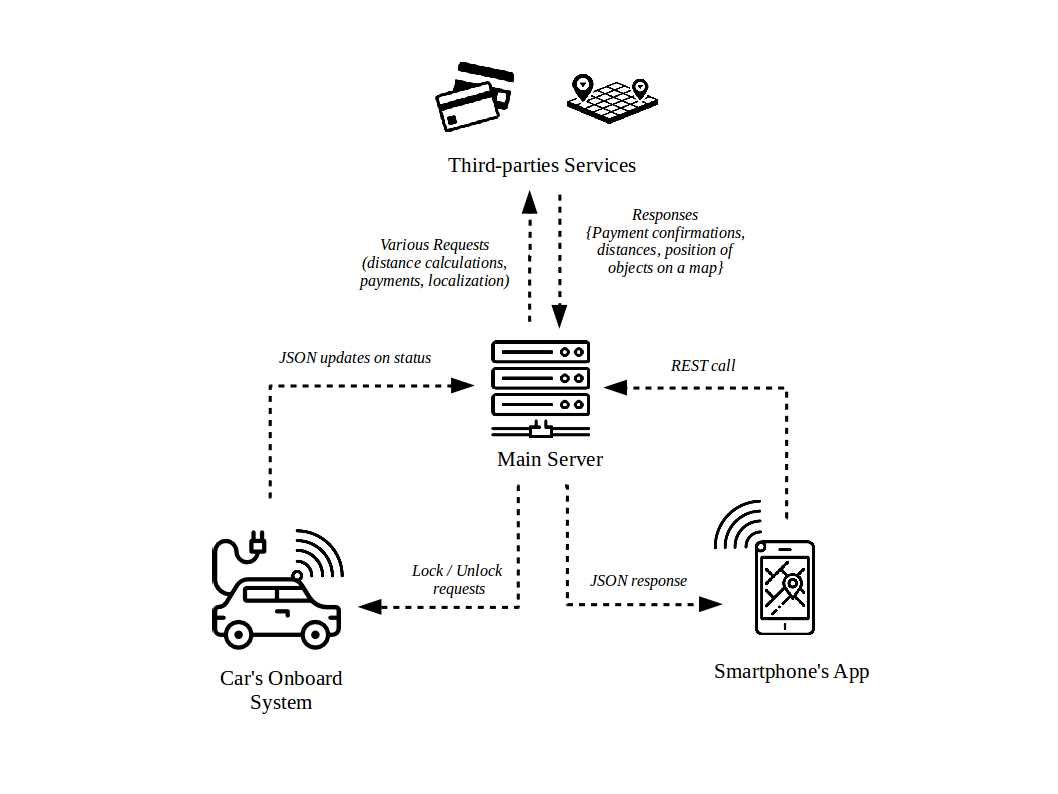
\includegraphics[width=1\textwidth]{proposed_system.png}
	\caption{Description of the proposed system.}
\end{figure}

\subsubsection{App Frontend}
The frontend is a thin app that relies on the smartphone's internet connections in order to work. Almost no operations can be performed with the app alone: all transactions are sent to the main server first, then processed and the result sent back to the app.

The app can be classified as a thin client.

\subsubsection{Centralized Backend}
The backend is the core of the system. Being able to process a lot of parallel operations, it can deal with all the requests coming from che clients ina reasonable amount of time (see Non Functionals Requirements). The backend is based on an MVC architecture and a REST API.

\subsubsection{Car's Onboard system}
The cars are equipped with an onboard system that monitors the status of the car, its location, and can send all the necessary informations to the main server. There won't be direct interactions between the car and the user's app.


\subsection{Actors and stakeholders}

\subsubsection{Actors}
The actors involved in our system are mainly \textbf{final users}, that is, people who are renting cars. Indeed the system needs support from a \textbf{technical team} that takes care of the digital infrastructure, and a \textbf{staff} that takes care of the cars in some special situations:
\begin{itemize} 
	\item Cars left far from the power grid with an empty battery, that needs to be charged in-place
	\item Cars left far from a safe parking area, that needs to be brought back to one of them
	\item Cars not plugged to the power grid, that needs to be plugged.
\end{itemize}

\subsubsection{Stakeholders}
The main stakeholder for our system are \textbf{users} themselves, who requires a easy-to-use service of electric cars sharing. Other stakeholders are the \textbf{city governement}, who supports our service as a way to improve sustainable mobility inside the city and takes care of the road infrastructures, and the \textbf{energy companies}, which provide power for the cars.

\subsection{Reference Documents}
\begin{itemize}
	\item \textit{Assignments AA 2016-2017.pdf} (Assignments document given by the teacher)
	\item \textit{IEEE Std 830-1998 IEEE Recommended Practice for Software Requirements Specifications}
	\item Other Sample documents:
		\begin{itemize}
			\item \textit{RASD sample from Oct. 20 lecture.pdf}
			\item \textit{Libra: An Economy-Driven Cluster Scheduler Software Requirements Specification}
		\end{itemize}
  \end{itemize}

 




\newpage
\section{Specific Requirements}

In this section we are going to illustrate the specific requirement of \pe.

We analyze the goals that the application should fullfill, then moving on functional and not functional requirements.

 \subsection{Goals}

\subsection{Domain Properties}

\subsection{Definitions,  acronyms,  abbreviations}
  	
  \begin{description}
  	\item[GPS]: Global Positioning System is a global navigation satellite system (GNSS) that provides location and time information in all weather conditions, anywhere on or near the Earth where there is an unobstructed line of sight to four or more GPS satellites.
  	\item[Frontend]
  	\item[Backend]
  \end{description}
  

\newpage
\section{Scenarios and Use Cases}

\subsection{Scenarios}

\subsection{Use Cases}


\newpage
\section{Alloy Model}

\newpage
\section{Hours}


\end{document}
